% 2007 年全国大纲卷Ⅱ理科第 19 题：正方形底面四棱锥
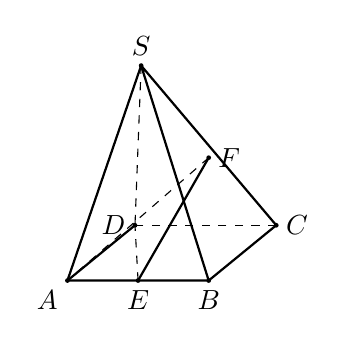
\begin{tikzpicture}[>=stealth,scale=0.78]
  \coordinate (A) at (0,0); \coordinate (B) at (2.3,0);
  \coordinate (C) at (3.4,0.9); \coordinate (D) at (1.1,0.9);
  \coordinate (S) at (1.2,3.5); \coordinate (E) at (1.15,0);
  \coordinate (F) at (2.3,2.0);
  \draw[thick] (A)--(B)--(C); \draw[dashed] (C)--(D); \draw[thick] (D)--(A);
  \draw[thick] (S)--(A) (S)--(B) (S)--(C);
  \draw[dashed] (S)--(D);
  \draw[thick] (E)--(F);
  \draw[dashed] (E)--(D) (F)--(A);
  \fill (S) circle (1.1pt) node[above] {$S$};
  \fill (A) circle (1.1pt) node[below left] {$A$};
  \fill (B) circle (1.1pt) node[below] {$B$};
  \fill (C) circle (1.1pt) node[right] {$C$};
  \fill (D) circle (1.1pt) node[left] {$D$};
  \fill (E) circle (1.1pt) node[below] {$E$};
  \fill (F) circle (1.1pt) node[right] {$F$};
\end{tikzpicture}
